\documentclass[a4paper,10pt]{article}
\usepackage[utf8]{inputenc}
\usepackage{amsmath,amsfonts,amssymb,graphicx,subfigure,mathtools}
\usepackage{amsmath}
\usepackage{rotating}
\usepackage{lscape}

\newcommand{\conj}[1]{\overline{#1}}

%MATRIX HELPER FUNCTIONS
\newcommand\coolover[2]{\mathrlap{\smash{\overbrace{\phantom{%
    \begin{matrix} #2 \end{matrix}}}^{\mbox{$#1$}}}}#2} 

\newcommand\coolunder[2]{\mathrlap{\smash{\underbrace{\phantom{%
    \begin{matrix} #2 \end{matrix}}}_{\mbox{$#1$}}}}#2}

\newcommand\coolleftbrace[2]{%
#1\left\{\vphantom{\begin{matrix} #2 \end{matrix}}\right.}

\newcommand\coolrightbrace[2]{%
\left.\vphantom{\begin{matrix} #1 \end{matrix}}\right\}#2}



%opening
\title{SPARC: SpArse Redundant Calibration}
\author{T.L. Grobler}

\begin{document}

\maketitle

%\begin{abstract}

%\end{abstract}

\begin{section}{No Name}

\begin{equation}
\boldsymbol{H} = 
\begin{bmatrix}
\boldsymbol{A} & \boldsymbol{B}\\
\boldsymbol{B}^* & \boldsymbol{A}^*
\end{bmatrix}
\end{equation}

With 

\begin{equation}
\boldsymbol{A} = 
\begin{bmatrix}
\boldsymbol{C} & \boldsymbol{D}\\
\boldsymbol{D^H} & \boldsymbol{E}
\end{bmatrix}
\end{equation}

\begin{equation}
\boldsymbol{B} = 
\begin{bmatrix}
\boldsymbol{F} & \boldsymbol{G}\\
\boldsymbol{G}^T & \boldsymbol{0}
\end{bmatrix}
\end{equation}

\begin{equation}
[\boldsymbol{C}]_{ij} = 
\begin{cases}
 \sum_{k \neq i} \left | g_k \right |^2 \left | y_{|i-k|} \right |^2 & \textrm{if} ~ i=j\\
 0 & \textrm{otherwise}
\end{cases}
\end{equation}

\begin{equation}
[\boldsymbol{D}]_{ij} = 
\begin{cases}
 g_i y_j^*  \left | g_{i+j} \right |^2  & \textrm{if} ~ i+j \leq N\\
 0 & \textrm{otherwise}
\end{cases}
\end{equation}

\begin{equation}
[\boldsymbol{E}]_{ij} = 
\begin{cases}
 \sum_{pq \in \mathcal{I}_i} \left | g_p \right |^2 \left | g_q \right |^2  & \textrm{if} ~ i=j\\
 0 & \textrm{otherwise}
\end{cases}
\end{equation}

\begin{equation}
[\boldsymbol{F}]_{ij} = 
\begin{cases}
 g_i g_j  \left | y_{|i-j|} \right |^2  & \textrm{if} ~ i \neq j\\
 0 & \textrm{otherwise}
\end{cases}
\end{equation}

\begin{equation}
[\boldsymbol{G}]_{ij} = 
\begin{cases}
 g_i y_j  \left | g_{i-j} \right |^2  & \textrm{if} ~ i > j\\
 0 & \textrm{otherwise}
\end{cases}
\end{equation}

Moreover, 

\begin{equation}
\mathcal{I}_i = \left\{pq|(q - p) = i \right\}
\end{equation}

The dimensions of the matrices:

\begin{enumerate}
\item $\boldsymbol{H}$: is a $(4N-2)\times(4N-2)$ or a $P \times P$ matrix. $N$ denotes the number of antennas and $P$ denotes the number of parameters. This matrix
contains $6N^2 - 2N - 2$ non-zero entries. It contains $16N^2 - 16N + 4$ entries. We can construct this matrix with $4N^2 -  4N$ or $\frac{1}{4} P^2 -1$ elementary operations.
\item $\boldsymbol{A}$: is a $(2N-1)\times(2N-1)$ matrix. This matrix has $N^2 + N - 1$ non-zero entries. We can construct this matrix with $2\frac{1}{2} (N^2 -  N)$ elementary operations.  
\item $\boldsymbol{B}$: is a $(2N-1)\times(2N-1)$ matrix. This matrix has $2N^2 - 2N$ non-zero entries. We can construct this matrix with $1\frac{1}{2} (N^2 -  N)$ elementary operations.
\item $\boldsymbol{C}$: is a $N\times N$ matrix. This matrix has $N$ non-zero entries. We can construct this matrix with $N^2-N$ elementary operations.
\item $\boldsymbol{D}$: is a $N \times (N-1)$ matrix. This matrix has $\frac{1}{2} (N^2 -  N)$ non-zero entries. We can construct this matrix with $\frac{1}{2} (N^2 -  N)$ elementary operations. 
\item $\boldsymbol{E}$: is a $(N-1) \times (N-1)$ matrix. This matrix has $(N-1)$ non-zero entries. We can construct this matrix with $\frac{1}{2} (N^2 -  N)$ elementary operations.  
\item $\boldsymbol{F}$: is a $N \times N$ matrix. This matrix has $N^2 - N$ non-zero entries. We can construct this matrix with $\frac{1}{2} (N^2 -  N)$ elementary operations.
\item $\boldsymbol{G}$: is a $N \times (N-1)$ matrix. This matrix has $\frac{1}{2} (N^2 -  N)$ non-zero entries. We can construct this matrix with $\frac{1}{2} (N^2 -  N)$ elementary operations.
\item $\boldsymbol{0}$: is a $(N-1) \times (N-1)$ all zero matrix. 
\end{enumerate}

We can construct $\boldsymbol{C}-\boldsymbol{G}$ in $O(N^2)$ 


The sparsity ratio of $\boldsymbol{H}$ is equal to
\begin{equation}
\gamma_N = \frac{10N^2-14N+6}{16N^2-16N+4} 
\end{equation}

The asymptotic sparsity ratio of $\boldsymbol{H}$ is equal to

\begin{equation}
\gamma = \lim_{N\rightarrow \infty}\frac{5N^2-7N+3}{8N^2-8N+2} = \frac{5}{8}
\end{equation}

Asymptotically the computational cost of the matrix-vector product between $\boldsymbol{H}$ and a vector of appropriate size is $O(P^2)$. However, the computational cost converges 
very slowly to its asymptotic value, and in general is equal to $O(P^{k_N})$, where $k_N < 2$.

\begin{eqnarray}
P^{k_N}_N &=& (1 - \gamma_N)P^2_N\\
k_N &=& \log_{P_N}(1 - \gamma_N) + 2\\
k &=& \lim_{N\rightarrow \infty} \log_{P_N}(1 - \gamma_N) + 2 = 2
\end{eqnarray}

Moreover,

\begin{eqnarray}
P^{c_N}_N &=& \frac{1}{4} P_N^2 -1\\
c_N &=& \log_{P_N}\left (\frac{1}{4} P_N^2-1 \right )\\
c &=& \lim_{N\rightarrow \infty} \log_{P_N}\left (\frac{1}{4} P_N^2-1\right ) = 2
\end{eqnarray}

NB $P_c$ IS WRONG HERE DID NOT TAKE INTO ACCOUNT THE CONJUGANTION OF $\boldsymbol{B}$ (need multiply its computational complexity by two).

\begin{figure}
  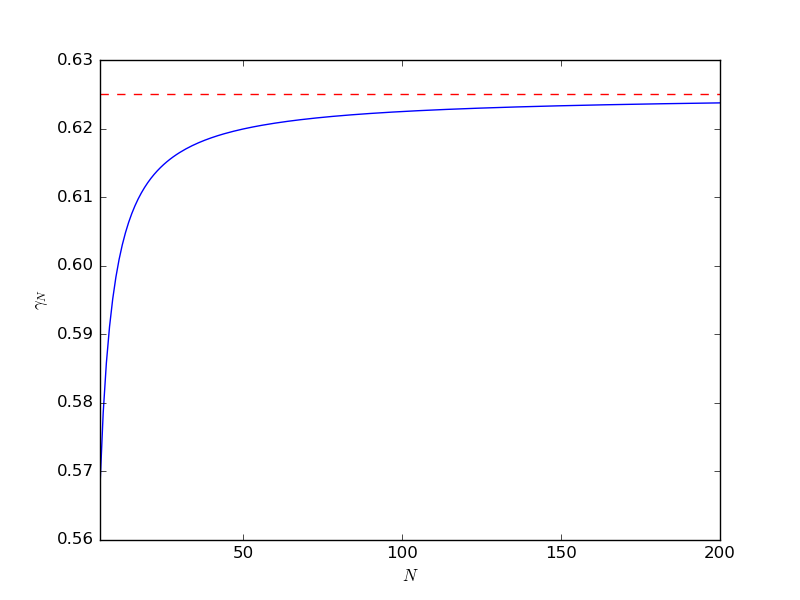
\includegraphics[width=\linewidth]{sparsity_factor.png}
  \caption{Sparsity factor $\gamma_N$.}
\end{figure}

\begin{figure}
  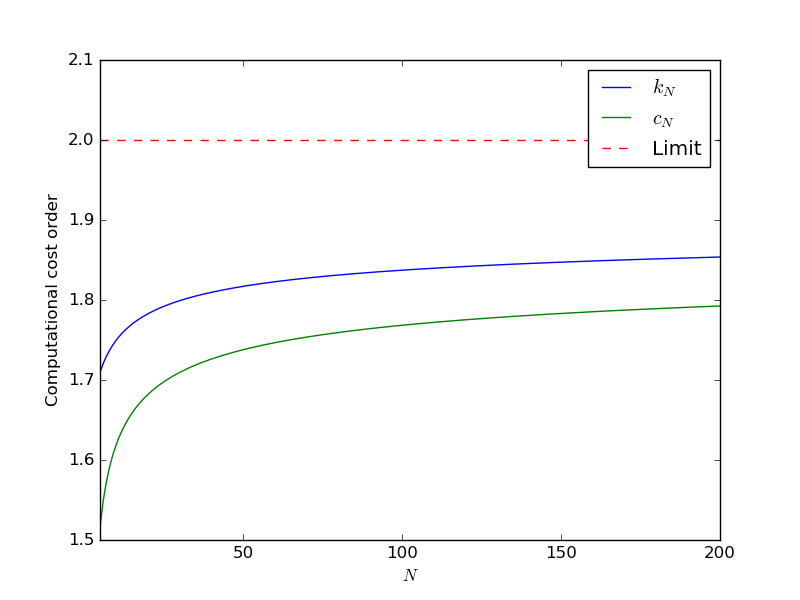
\includegraphics[width=\linewidth]{k_N.png}
  \caption{Computation complexity order of matrix-vector product and construction.}
\end{figure}

THE POTENTIAL GENERAL FORMULATION

Let $\phi_{pq}:\mathbb{N}^2\rightarrow\mathbb{N}^+$ be the mapping that maps antenna indices to the redundant spacing indices of the array. Also note that this mapping is not symmetric as 
$\phi_{pq} = 0$ if $p>q$. Moreover, let

\begin{equation}
\psi_{ij} = 
\begin{cases}
q~\textrm{if}~\exists! ~ q \in \mathbb{N} ~ s.t. ~(\phi_{iq} = j)\\
0~\textrm{otherwise}
\end{cases}
\end{equation},

\begin{equation}
\xi_{ij} = 
\begin{cases}
p~\textrm{if}~\exists! ~ p \in \mathbb{N} ~ s.t. ~(\phi_{pi} = j)\\
0~\textrm{otherwise}
\end{cases}
\end{equation}

and

\begin{equation}
\zeta_{ij} = 
\begin{cases}
\phi_{ij}~\textrm{if}~i<j\\
\phi_{ji}~\textrm{if}~i>j\\
0~\textrm{otherwise}
\end{cases}
\end{equation}

\begin{equation}
\boldsymbol{H} = 
\begin{bmatrix}
\boldsymbol{A} & \boldsymbol{B}\\
\boldsymbol{B}^* & \boldsymbol{A}^*
\end{bmatrix}
\end{equation}

With 

\begin{equation}
\boldsymbol{A} = 
\begin{bmatrix}
\boldsymbol{C} & \boldsymbol{D}\\
\boldsymbol{D^H} & \boldsymbol{E}
\end{bmatrix}
\end{equation}

\begin{equation}
\boldsymbol{B} = 
\begin{bmatrix}
\boldsymbol{F} & \boldsymbol{G}\\
\boldsymbol{G}^T & \boldsymbol{0}
\end{bmatrix}
\end{equation}

\begin{equation}
[\boldsymbol{C}]_{ij} = 
\begin{cases}
 \sum_{k \neq i} \left | g_k \right |^2 \left | y_{\zeta_{ik}} \right |^2 & \textrm{if} ~ i=j\\
 0 & \textrm{otherwise}
\end{cases}
\end{equation}

\begin{equation}
[\boldsymbol{D}]_{ij} = 
\begin{cases}
 g_i y_j^*  \left | g_{\psi_{ij}} \right |^2  & \textrm{if} ~ \psi_{ij}\neq0\\
 0 & \textrm{otherwise}
\end{cases}
\end{equation}

\begin{equation}
[\boldsymbol{E}]_{ij} = 
\begin{cases}
 \sum_{pq \in \mathcal{I}_i} \left | g_p \right |^2 \left | g_q \right |^2  & \textrm{if} ~ i=j\\
 0 & \textrm{otherwise}
\end{cases}
\end{equation}

\begin{equation}
[\boldsymbol{F}]_{ij} = 
\begin{cases}
 g_i g_j  \left | y_{\zeta_{ij}} \right |^2  & \textrm{if} ~ (i \neq j)\\
 0 & \textrm{otherwise}
\end{cases}
\end{equation}

\begin{equation}
[\boldsymbol{G}]_{ij} = 
\begin{cases}
 g_i y_j  \left | g_{\xi_{ij}} \right |^2  & \textrm{if} ~ (\xi_{ij}\neq0)\\
 0 & \textrm{otherwise}
\end{cases}
\end{equation}

Moreover, 

\begin{equation}
\mathcal{I}_i = \left\{pq\in\mathbb{N}^2|(\phi_{pq} = i) \right\}.
\end{equation}

FOR AN EW ARRAY WE HAVE

\begin{equation}
\phi_{ij} = 
\begin{cases}
j - i & \textrm{if}~i<j\\
0 & \textrm{otherwise}
\end{cases}
\end{equation}

\begin{equation}
\psi_{ij} = 
\begin{cases}
i+j & \textrm{if}~(0<i<N)\wedge(0<j<N)\wedge(0< i+j \leq N)\\
0 & \textrm{otherwise}
\end{cases}
\end{equation}

\begin{equation}
\zeta_{ij} = 
\begin{cases}
j - i & \textrm{if}~i<j\\
i - j & \textrm{if}~i>j\\
0 & \textrm{otherwise}
\end{cases}
\end{equation}

\begin{equation}
\xi_{ij} = 
\begin{cases}
i-j & (0<i<N)\wedge(0<j<N)\wedge(i>j)\\
0 & \textrm{otherwise}
\end{cases}
\end{equation}

LINCAL

\begin{equation}
\boldsymbol{H} =
\begin{bmatrix}
\boldsymbol{\mathcal{A}} & \boldsymbol{\mathcal{B}}\\
\boldsymbol{\mathcal{B}}^H & \boldsymbol{\mathcal{C}}
\end{bmatrix}
\end{equation}

\begin{equation}
\boldsymbol{\mathcal{A}} =
\begin{bmatrix}
\boldsymbol{\mathcal{D}} & \boldsymbol{\mathcal{E}}\\
\boldsymbol{\mathcal{E}}^H & \boldsymbol{\mathcal{F}}
\end{bmatrix}
\end{equation}

\begin{equation}
\boldsymbol{\mathcal{B}} =
\begin{bmatrix}
\boldsymbol{\mathcal{G}} & j\boldsymbol{\mathcal{G}}\\
\boldsymbol{\mathcal{H}}^H & j\boldsymbol{\mathcal{H}}
\end{bmatrix}
\end{equation}

\begin{equation}
\boldsymbol{\mathcal{C}} =
\begin{bmatrix}
\boldsymbol{\mathcal{I}} & j\boldsymbol{\mathcal{I}}\\
-j\boldsymbol{\mathcal{I}}^H & \boldsymbol{\mathcal{I}}
\end{bmatrix}
\end{equation}

\begin{equation}
[\boldsymbol{\mathcal{D}}]_{ij} = 
\begin{cases}
|g_i|^2|y_{\zeta_{ij}}|^2|g_j|^2 & i\neq j\\
\sum_{k \neq i} |g_k|^2|g_i|^2|y_{\zeta_{ij}}|^2 & i = j
\end{cases}
\end{equation}

\begin{equation}
[\boldsymbol{\mathcal{E}}]_{ij} =
\begin{cases}
j \delta_{ij} |g_i|^2|y_{\zeta_{ij}}|^2|g_j|^2 & i\neq j\\
-j \sum_{k \neq i} \delta_{ik} |g_k|^2|g_i|^2|y_{\zeta_{ij}}|^2 & i = j
\end{cases}
\end{equation}

\begin{equation}
[\boldsymbol{\mathcal{F}}]_{ij} =
\begin{cases}
 -|g_i|^2|y_{\zeta_{ij}}|^2|g_j|^2 & i\neq j\\
 \sum_{k \neq i} \delta_{ik} |g_k|^2|g_i|^2|y_{\zeta_{ij}}|^2 & i = j
\end{cases}
\end{equation}

\begin{equation}
[\boldsymbol{\mathcal{G}}]_{ij} = \sum_{pq\in\mathcal{I}_{ij}} |g_p|^2|g_q|^2|y_{\zeta_{pq}}|^2
\end{equation}

\begin{equation}
[\boldsymbol{\mathcal{H}}]_{ij} = j \sum_{pq\in\mathcal{I}_{ij}} \widehat{\delta}_{pqi} |g_p|^2|g_q|^2|y_{\zeta_{pq}}|^2
\end{equation}

\begin{equation}
 [\boldsymbol{\mathcal{K}}]_{ij} = 
\begin{cases}
0 & i\neq j\\
\sum_{pq\in\mathcal{I}_{i}} |g_p|^2|g_q|^2|y_{\zeta_{pq}}|^2 & i=j
\end{cases}
\end{equation}

\begin{equation}
\mathcal{I}_{ij} = \{il\in\mathcal{B}|\zeta_{il}=j\}\cup\{li\in\mathcal{B}|\zeta_{li}=j\} 
\end{equation}

\begin{equation}
\mathcal{B} = \{st\in\mathbb{N}^2|s<t \wedge s<N \wedge t<N\}
\end{equation}

\begin{equation}
\widehat{\delta}_{pqi} = 
\begin{cases}
-1 & p = i\\
1 & q = i\\
0 & \textrm{otherwise}
\end{cases}
\end{equation}

\begin{equation}
\mathcal{I}_i = \{pq\in\mathcal{B}|\zeta_{pq}=i\} 
\end{equation}

\begin{equation}
\delta_{ij} =
\begin{cases}
-1 & i<j\\
1 & \textrm{otherwise}
\end{cases}
\end{equation}

LINCAL NEW (CORRECT VERSION)

\begin{equation}
\boldsymbol{H} =
\begin{bmatrix}
\boldsymbol{\mathcal{A}} & \boldsymbol{\mathcal{B}}\\
\boldsymbol{\mathcal{B}}^T & \boldsymbol{\mathcal{C}}
\end{bmatrix}
\end{equation}

\begin{equation}
\boldsymbol{\mathcal{A}} =
\begin{bmatrix}
\boldsymbol{\mathcal{D}} & \boldsymbol{0}\\
\boldsymbol{0} & \boldsymbol{\mathcal{T}}\odot\boldsymbol{\mathcal{D}}
\end{bmatrix}
\end{equation}

\begin{equation}
[\boldsymbol{\mathcal{D}}]_{ij} = 
\begin{cases}
2|g_i|^2|y_{\zeta_{ij}}|^2|g_j|^2 & i\neq j\\
2\sum_{k \neq i} |g_k|^2|g_i|^2|y_{\zeta_{ik}}|^2 & i = j
\end{cases}
\end{equation}

\begin{equation}
\boldsymbol{\mathcal{T}} = 2\boldsymbol{I}-\boldsymbol{1}
\end{equation}

\begin{equation}
\boldsymbol{\mathcal{B}} =
\begin{bmatrix}
\boldsymbol{\mathcal{E}} & \boldsymbol{0}\\
\boldsymbol{0} & \boldsymbol{\mathcal{F}}
\end{bmatrix}
\end{equation}

\begin{equation}
[\boldsymbol{\mathcal{E}}]_{ij} = 2\sum_{pq\in\mathcal{I}_{ij}} |g_p|^2|g_q|^2|y_{\zeta_{pq}}|^2
\end{equation}

\begin{equation}
[\boldsymbol{\mathcal{F}}]_{ij} = 2\sum_{pq\in\mathcal{I}_{ij}} \delta_{pq}^i |g_p|^2|g_q|^2|y_{\zeta_{pq}}|^2
\end{equation}



\begin{equation}
\mathcal{I}_{ij} = \{il\in\mathcal{B}|\zeta_{il}=j\}\cup\{li\in\mathcal{B}|\zeta_{li}=j\} 
\end{equation}

\begin{equation}
\mathcal{B} = \{st\in\mathbb{N}^2|s<t \wedge s<N \wedge t<N\}
\end{equation}

\begin{equation}
\delta_{pq}^i = 
\begin{cases}
1 & p = i\\
-1 & q = i\\
0 & \textrm{otherwise}
\end{cases}
\end{equation}

\begin{equation}
\boldsymbol{\mathcal{C}} =
\begin{bmatrix}
\boldsymbol{\mathcal{G}} & \boldsymbol{0}\\
\boldsymbol{0} & \boldsymbol{\mathcal{G}}
\end{bmatrix}
\end{equation}

\begin{equation}
 [\boldsymbol{\mathcal{G}}]_{ij} = 
\begin{cases}
0 & i\neq j\\
2\sum_{pq\in\mathcal{I}_{i}} |g_p|^2|g_q|^2|y_{\zeta_{pq}}|^2 & i=j
\end{cases}
\end{equation}

\begin{equation}
\mathcal{I}_i = \{pq\in\mathcal{B}|\zeta_{pq}=i\} 
\end{equation}

REDUNDANT STEFCAL DERIVATION

\begin{equation}
\boldsymbol{J}^H\breve{\boldsymbol{v}} = \widetilde{\boldsymbol{H}}\breve{\boldsymbol{z}} 
\end{equation}

\begin{equation}
\frac{1}{3} \boldsymbol{J}\breve{\boldsymbol{z}} = \breve{\boldsymbol{v}}
\end{equation}

\begin{equation}
\widetilde{\boldsymbol{H}} = \boldsymbol{I}\odot\boldsymbol{H} 
\end{equation}

\begin{eqnarray}
\begin{bmatrix} \Delta \boldsymbol{z}\\ \Delta \conj{\boldsymbol{z}} \end{bmatrix} &=& (\boldsymbol{J}^H\boldsymbol{J})^{-1} \boldsymbol{J}^H(\breve{\boldsymbol{d}}-\breve{\boldsymbol{v}})\\
&=& (\boldsymbol{J}^H\boldsymbol{J})^{-1}\boldsymbol{J}^H\breve{\boldsymbol{d}} - \frac{1}{3}(\boldsymbol{J}^H\boldsymbol{J})^{-1}(\boldsymbol{J}^H\boldsymbol{J})\breve{\boldsymbol{z}}\\
\breve{\boldsymbol{z}}_{k+1} &=& (\boldsymbol{J}^H\boldsymbol{J})^{-1}\boldsymbol{J}^H\breve{\boldsymbol{d}} + \frac{2}{3}\breve{\boldsymbol{z}}_k  
\end{eqnarray}

Gauss-Newton:

\begin{eqnarray}
\begin{bmatrix} \Delta \boldsymbol{z}\\ \Delta \conj{\boldsymbol{z}} \end{bmatrix} &\approx& \widetilde{\boldsymbol{H}}^{-1}\boldsymbol{J}^H(\breve{\boldsymbol{d}}-\breve{\boldsymbol{v}})\\ 
&=& \widetilde{\boldsymbol{H}}^{-1}\boldsymbol{J}^H\breve{\boldsymbol{d}} -  \widetilde{\boldsymbol{H}}^{-1}\widetilde{\boldsymbol{H}}\breve{\boldsymbol{z}}\\
\breve{\boldsymbol{z}}_{k+1} &\approx& \widetilde{\boldsymbol{H}}^{-1}\boldsymbol{J}^H\breve{\boldsymbol{d}}
\end{eqnarray}

Levenberg-Marquardt:

\begin{eqnarray}
\breve{\boldsymbol{z}}_{k+1} &\approx& \frac{1}{1+\lambda}\widetilde{\boldsymbol{H}}^{-1}\boldsymbol{J}^H\breve{\boldsymbol{d}} + \frac{\lambda}{1+\lambda} \breve{\boldsymbol{z}}_k\\
 &=& \alpha \widetilde{\boldsymbol{H}}^{-1}\boldsymbol{J}^H\breve{\boldsymbol{d}} + (1-\alpha)\breve{\boldsymbol{z}}_k 
\end{eqnarray}

with $\alpha = \frac{1}{1+\lambda}$. Moreover $\lambda = \frac{1-\alpha}{\alpha}$. So in Marthi and Chengular (2014) they use an $\alpha$ of 0.3, which corresponds to an LM damping factor $\lambda$
of $2\frac{1}{3}$.



%\[  \vphantom{% phantom stuff for correct box dimensions
%    \begin{matrix}
%    \overbrace{XYZ}^{\mbox{$R$}}\\ \\ \\ \\ \\ \\ 
%    \underbrace{pqr}_{\mbox{$S$}}
%    \end{matrix}}%
%\begin{matrix}% matrix for left braces
%\vphantom{a}\\ 
%\coolleftbrace{A}{e \\ y\\ y}\\
%\coolleftbrace{B}{y \\i \\ m}
%\end{matrix}%
%\begin{bmatrix}
%a & \coolover{R}{b & c & d} & x & \coolover{Z}{x & x}\\
%e & f & g & h & x & x & x \\
%y & y & y & y & y & y & y \\
%y & y & y & y & y & y & y \\
%y & y & y & y & y & y & y \\
%i & j & k & l & x & x & x \\
%m &  \coolunder{S}{n & o}  & \coolunder{W}{p & x & x} & x
%\end{bmatrix}%
%\begin{matrix}% matrix for right braces 
%\coolrightbrace{x \\ x \\ y\\ y}{T}\\
%\coolrightbrace{y \\ y \\ x }{U}
%\end{matrix}\]

\begin{equation}
\boldsymbol{J}^H\breve{\boldsymbol{d}} = 
\begin{bmatrix}
\sum_{k\neq i } g_k x_{ik}d_{ik}\\
\sum_{pq \in \mathcal{I}_j} \conj{g}_p g_q d_{pq}\\
\downarrow^{*}
\end{bmatrix}
\begin{matrix}% matrix for right braces 
\coolrightbrace{\sum g_k x_{\zeta_{ik}}d_{ik}}{i = 1\cdots N}\\
\coolrightbrace{\sum \conj{g}_p g_q d_{pq}}{j = 1\cdots L}\\
\vphantom{\downarrow^{*}}
\end{matrix}
\end{equation}

\begin{equation}
x_{ik} = 
\begin{cases}
\conj{y}_{\zeta_{ik}} & \textrm{if}~k > i\\
y_{\zeta_{ik}} & \textrm{otherwise}
\end{cases}
\end{equation}

Which implies that 

\begin{equation}
g_{i}^{k+1} = \alpha \frac{\sum_{k\neq i } g_k x_{ik}d_{ik}}{|g_k|^2|y_{\zeta_{ik}}|^2} + (1-\alpha) g_i^k 
\end{equation}

\begin{equation}
y_{i}^{k+1} = \alpha \frac{\sum_{pq \in \mathcal{I}_j} \conj{g}_p g_q d_{pq}}{\sum_{pq \in \mathcal{I}_j}|g_p|^2|g_q|^2} + (1-\alpha) y_i^k 
\end{equation}

\begin{equation}
\boldsymbol{J} =
\begin{bmatrix}
\boldsymbol{\mathcal{M}} & \boldsymbol{\mathcal{N}}\\
\boldsymbol{\mathcal{N}}^* & \boldsymbol{\mathcal{M}}^*
\end{bmatrix}
\end{equation}

\begin{equation}
\boldsymbol{\mathcal{M}} = 
%\vphantom{% phantom stuff for correct box dimensions
%    \begin{matrix}
%    \overbrace{XYZ}^{\mbox{$y_{\zeta_{pq}} \conj{g}_q \delta_p^j$}} 
%    \end{matrix}}
\begin{bmatrix}
\coolover{{\scriptstyle j=1,\ldots,N}}{y_{\zeta_{pq}} \conj{g}_q \delta_p^j} & \coolover{{\scriptstyle k=1,\ldots,L}}{g_p\conj{g}_q\delta_{\zeta_{pq}}^k}
\end{bmatrix}
\begin{matrix}% matrix for right braces 
\coolrightbrace{g_p\conj{g}_q\delta_{\zeta_{pq}}^k}{{\scriptstyle[pq] = 1,\ldots,B~(p<q)}}
\end{matrix}
\end{equation}

\begin{equation}
\boldsymbol{\mathcal{N}} = 
%\vphantom{% phantom stuff for correct box dimensions
%    \begin{matrix}
%    \overbrace{XYZ}^{\mbox{$y_{\zeta_{pq}} \conj{g}_q \delta_p^j$}} 
%    \end{matrix}}
\begin{bmatrix}
\coolover{{\scriptstyle j=1,\ldots,N}}{g_p y_{\zeta_{pq}} \delta_q^j} & \boldsymbol{0}
\end{bmatrix}
\begin{matrix}% matrix for right braces 
\coolrightbrace{g_p\conj{g}_q\delta_{\zeta_{pq}}^k}{{\scriptstyle[pq] = 1,\ldots,B~(p<q)}}
\end{matrix}
\end{equation}




\begin{equation}
\delta_x^y=
\begin{cases}
1 & \textrm{if}~x=y\\
0 & \textrm{otherwise}
\end{cases}
\end{equation}







%\begin{equation}
%\begin{matrix}% matrix for right braces 
%\coolrightbrace{x \\ x \\ y\\ y}{T}\\
%\coolrightbrace{y \\ y \\ x }{U}
%\end{matrix}
%\end{equation}






\end{section}
\end{document}
 